\chapter{Bestaande systemen}

De opgeslagen informatie neemt elke dag enorm toe. Ontdekken van patronen en trends uit deze steeds groeiende data is een taak die steeds moeilijker wordt. Bepaalde technieken kunnen gebruikt worden om het probleem op te lossen. De basistechniek daarbij is \textit{data mining} (zie \ref{data-mining}), waarvan toepassingen o.a. \textit{text mining} (zie \ref{text-mining}) en \textit{web mining} zijn \cite{Nasa2012}. 

\section{Data mining}\label{data-mining}
Data mining werd in 1980 voor het eerst gebruikt om data om te zetten naar kennis. Het doel van data mining is om impliciete, vooraf onbekende trends en patronen uit databases te halen. Daarbij wordt gebruik gemaakt van verschillende technieken: classificatie, clustering, neurale netwerken, beslissingsbomen, etc. 
\\Data mining is deel van het \textit{knowledge discovering process} of \textit{knowledge discovery in databases} (KDD). Dit proces bestaat uit verschillende stappen:
\begin{enumerate}
	\item Begrijpen van business: de objectieven en verwachtingen worden gedefinieerd.
	\item Begrijpen van data: data wordt uit het data warehouse geselecteerd op basis van de gedefinieerde objectieven en verwachtingen.
	\item Voorbereiden van data: de kwaliteit van de data wordt verbeterd.
	\item Modelleren van data: een data mining algoritme wordt geselecteerd en toegepast op de data die voorbereid werd in de vorige stap.
	\item Evaluatie: de relaties en patronen worden geanalyseerd en geldige patronen volgens de vooraf opgestelde doelen worden geselecteerd.
	\item Visuele representatie: de kennis die ontdekt is wordt visueel voorgesteld. Deze resultaten kunnen opgeslagen en samengevoegd worden, om de business vooruit te helpen.
\end{enumerate}

\section{Text mining}\label{text-mining}
\textit{Content recognition} of \textit{text mining} verwijst naar de extractie van interessante informatie en kennis uit ongestructureerde tekst. Het probeert om de verborgen informatie te onthullen door middel van methodes die enerzijds met een groot aantal woorden en structuren in natuurlijke taal kunnen omgaan en anderzijds vaagheid en onzekerheid kunnen verwerken. Text mining kan naast met gestructureerde data (zoals de data die in data mining verwerkt wordt) ook werken met ongestructureerde of semi-gestructureerde data zoals e-mails, volledige tekstdocumenten, HTML bestanden, etc. Text mining wordt daarom beschreven als een interdisciplinaire methode op basis van \textit{information retrieval}\footnote{Het vinden van documenten die antwoorden bevatten op vragen, maar niet het vinden van de antwoorden zelf.},\textit{ machine learning}, statistiek, computationele taalkunde en vooral data mining  \cite{Hotho2005}. 

Om grote collecties van documenten te verwerken, moeten tekstdocumenten vooraf verwerkt worden om de informatie op te slaan in een datastructuur die beter geschikt is dan een tekstbestand. De meeste text mining-methodes gaan ervan uit dat een tekstdocument voorgesteld kan worden als een set van woorden (\textit{bag-of-words} representatie, zie \ref{bag-of-words}). Ondertussen bestaan echter methodes die proberen om de syntactische structuur of de semantiek in de tekst uit te buiten. Op die manier kan de belangrijkheid van een woord achterhaald worden. Hiervoor wordt vaak een vector representatie gebruikt, die voor elk woord een numeriek gewicht bijhoudt. Enkele belangrijke modellen die hiervoor gebruikt worden zijn het vector space model \cite{Salton1975}, het probabilistische model \cite{ROBERTSON1977} en het logische model \cite{Rigsbergen1986}. In deze masterproef wordt gebruik gemaakt van het vector space model (zie \ref{vector-space-model}).


\subsection{\textit{Preprocessing} van tekstdocumenten}\label{bag-of-words}
Om alle woorden te verkrijgen die gebruikt worden in een bepaalde tekst, wordt een \textit{tokenization}\label{tokenization} proces toegepast. Dit zorgt ervoor dat een tekstdocument gesplitst wordt in een stroom van woorden door alle leestekens te verwijderen en alle tabs en niet-tekstuele karakters door spaties te vervangen. De set van verschillende woorden uit alle tekstdocumenten wordt samengevoegd tot het woordenboek van de documentencollectie. Het tokenization proces dat hier gebruikt wordt is de \textit{N-Gram tokenizer} \cite{McNamee2004}. Deze geeft ons de mogelijkheid om eventueel twee of drie woorden samen te nemen en die als \'e\'en woord in onze documentencollectie te zien. Dit kan voordeel geven bij o.a. personennamen, welke vaak bestaan uit twee woorden die voor een tekst belangrijk zouden kunnen zijn. Uiteraard wordt een eigennaam ook opgepikt indien alle woorden apart beschouwd worden.

Om de grootte van het woordenboek en dus de dimensionaliteit van de beschrijving van de documentencollectie te verkleinen, wordt de set van woorden eerst gereduceerd door het toepassen van filters of \textit{stemming}salgoritmes. 

Filters verwijderen woorden van het woordenboek en dus uit de documenten. De filtering die hier wordt toegepast is stopwoordfiltering. Stopwoorden zijn woorden die weinig of geen inhoud hebben. Voorbeelden zijn lidwoorden, verbindingswoorden, voorzetsels, etc. 

Stemmingsalgoritmes proberen een woord om te vormen tot de standaardvorm van dat woord. Dit doen ze bijvoorbeeld door meervouden van zelfstandige naamwoorden naar het enkelvoud om te zetten of door werkwoorden naar hun stam te vereenvoudigen. Het stemmingalgoritme dat hier gebruikt wordt is Porters stemming algoritme voor de Nederlandse taal \cite{Kraaij1994}. Het is een implementatie van Porters stemming algoritme \cite{Porter1980}, dat origineel enkel voor de Engelse taal werd ontworpen.

\subsection{Vector space model}\label{vector-space-model}
Ondanks de simpele datastructuur zorgt het vector space model ervoor dat grote collecties documenten effici\"ent kunnen geanalyseerd worden. Het representeert documenten als vectors in een $m$-dimensionale ruimte. Elk document $d$ uit de documentencollectie is beschreven als een numerieke\textit{ feature vector} $w(d) = (x(d,t_1),...,x(d,t_m))$ waarbij $T=\{t_1,...,t_m\}$ het woordenboek voorstelt. De hoofdtaak van de vector space representatie van documenten is het vinden van een geschikte encodering van de feature vector. 

Elk element van de vector representeert meestal een woord (of groep van woorden) van de documentencollectie. De simpelste manier om een document te encoderen is om \textit{binary term} vectoren te gebruiken. Als een woord voorkomt in het document wordt het corresponderende element op \'e\'en gezet, komt het niet voor dan is het nul. De encodering wordt zo herleid tot een simpele Booleaanse vergelijking. Hierbij wordt de belangrijkheid van elk woord als gelijkwaardig beschouwd. 

Om de performantie te verbeteren worden \textit{term weighting schemes} gebruikt \cite{Salton1988}. Het gewicht dat toegekend wordt aan een woord reflecteert de belangrijkheid of relevantie van dat woord in een specifiek document of collectie. Een woord met hoge frequentie in bepaalde documenten, maar dat weinig of niet voorkomt in de volledige documentencollectie wordt een groot gewicht toebedeeld. Een gewicht $w(d,t)$ voor term $t$ in document $d$ wordt berekend als de term frequency $tf(d,t)$ vermenigvuldigd met de inverse document frequency $idf(t)$ - gedefinieerd als $idf(t)=\log{\frac{N}{n_t}})$. Dit beschrijft de specifiteit van een bepaalde term in een documentencollectie. 

Naast term frequency en inverse document frequency wordt een normalisatie toegepast om ervoor te zorgen dat alle documenten dezelfde kans hebben om gevonden te worden, onafhankelijk van hun lengte. Deze techniek heeft zijn nut reeds bewezen in de praktijk . 
\begin{equation}\label{eq:tfidf}
w(d,t) = \frac{tf(dt)\log{\frac{N}{N_t}})}{\sqrt{\sum_{j=1}^{m}tf(d,t_j)^2(log(\frac{N}{n_{t_j}}))^2}}
\end{equation}
Hierbij stelt $N$ de grootte van de documentencollectie $D$ voor en is $n_t$ het aantal documenten in $D$ dat term $t$ bevat.

\subsection{Feature selection}
Feature selection of attribute selection zorgt ervoor dat attributen die niet relevant zijn verwijderd worden. Dit zorgt er o.a. voor dat de dataset kleiner wordt, waardoor minder rekenkracht en zoekruimte vereist is bij de effectieve verwerking van het vector model. Volgens \cite{Liu2005} is het \'e\'en van de meest belangrijke en meest gebruikte technieken voor data preprocessing bij data mining. Het reduceert het aantal features, het verwijdert irrelevante of redundante data en het zorgt er bijgevolg voor dat data mining algoritmes sneller werken. Het zorgt er o.m. ook voor dat de voorspelde accuraatheid en begrijpbaarheid van de resultaten verbeterd wordt. Feature selection is vooral interessant bij text mining, omdat er een hoge dimensionaliteit is van de features en er veel irrelevante features voorkomen.

Als de dimensionaliteit van een domein bovendien vergroot wordt, verhoogt het aantal features $N$. Een optimale subset van features vinden is zeer moeilijk en veel problemen gerelateerd aan feature selection zijn NP-moeilijk. Volgens \cite{Liu2005} bestaat een typisch feature selection proces uit vier stappen (zie figuur \ref{fig:feature-selection}); subset generatie, subset evaluatie, stopcriterium en resultatenvalidatie.

\begin{figure}[h]
	\caption{Vier stappen in feature selection}
	\label{fig:feature-selection}
	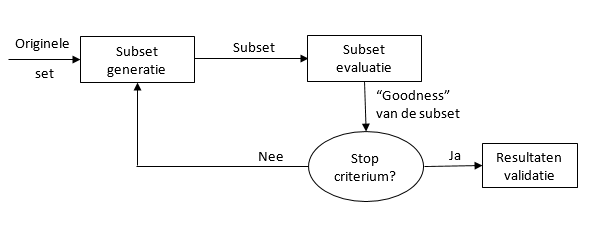
\includegraphics[width=\textwidth]{fig/feature-selection}
\end{figure}

Subset generatie is een zoekprocedure die kandidaat feature subsets produceert voor evaluatie met een bepaalde zoekstrategie. Elke kandidaat subset wordt ge\"evalueerd en vergeleken met de vorige beste volgens een bepaald criterium. Als de nieuwe subset beter is, wordt de vorige beste subset vervangen. Dit proces wordt herhaald tot een bepaald stopcriterium is bereikt. Dan wordt de geselecteerde beste subset gevalideerd met voorkennis of via verschillende tests op andere datasets. Feature selection is zowel interessant voor classificatie als clustering. 


\section{Data mining methodes voor tekst}
De hoofdreden om data mining methodes in te zetten voor documentencollecties is om ze te structureren. Een structuur kan het gemakkelijker maken voor de gebruiker om een documentencollectie te raadplegen. Bestaande methodes die toestaan om documentencollecties te structureren proberen om kernwoorden aan documenten te koppelen op basis van een gegeven set kernwoorden (via classificatie of categorisatie, zie \ref{classificatie}) of proberen de documentencollectie automatisch te structureren in groepen van gelijkaardige documenten (\textit{clustering}, zie \ref{clustering}).


\subsection{Classificatie}\label{classificatie}
Classificatie of categorisatie heeft als doel om voorgedefinieerde klasses toe te kennen aan tekstdocumenten. Het is een \textit{supervised} techniek\footnote{Een set van input-output voorbeelden worden gebruikt om het model te trainen, om zo nieuwe documenten te kunnen classifiseren.} die de \textit{classifier} traint op basis van gekende voorbeelden en zijn opgesteld model vervolgens gebruikt om ongekende voorbeelden automatisch te categoriseren \cite{Nasa2012}. 



\subsection{Clustering}\label{clustering}
Clustering is een \textit{unsupervised} techniek waar geen patronen voorgedefinieerd zijn. De methode is gebasseerd op een concept dat gelijkaardige documenten of teksten in dezelfde cluster groepeert. Elke cluster bevat dus een aantal documenten. De clustering wordt als beter beschouwd indien de inhoud van de documenten intra-cluster meer gelijkheid vertoont dan de inhoud van de documenten inter-cluster.

Clustering wordt gebruikt om gelijkaardige documenten te groeperen, maar verschilt van classificatie omdat documenten bij clustering on-the-fly ingedeeld worden in clusters, in plaats van in vooraf gedefinieerde klasses of topics.

\section{WEKA}
WEKA (Waikato Environment for Knowledge Analysis) is een tool voor datamining ontwikkeld in de programmeertaal Java. Het bestaat uit een grafische werkomgeving  voor het uitvoeren van de nodige stappen bij datamining, een CLI en is volledig ondersteund voor gebruik binnen een eigen Java-programma. Het helpt bij de preprocessing van data en bevat heel wat algoritmes voor clustering, classificatie, regressie-analyse, visualisatie en feature selection.

De versie van WEKA die gebruikt wordt in deze masterproef is 3.6.13, de op heden laatste stabiele versie.

\textbf{TODO: meer + referentie}

\section{Datasets}
\subsection{Het Laatste Nieuws}
De datasets die in eerste instantie gebruikt zullen worden zijn afkomstig van Het Laatste Nieuws, een populaire online en offline krant in Belgi\"e. De artikels die gebruikt worden komen van de online krant en werden gedownload via het archief. Om rekenkracht te besparen tijdens het onderzoek worden twee datasets gebruikt; een dataset met alle artikels van januari 2008 (10126 artikels) en een dataset met alle artikels van het jaar 2008 (82753 artikels).

Elk artikel behoort toe aan een boomstructuur van categorie\"en met twee niveaus. Het aantal hoofdcategorie\"en varieert tussen elf en twaalf (tijdens 2008 werd 1 hoofdcategorie toegevoegd in vergelijking met januari 2008). Voor de dataset van januari 2008 kunnen de hoofdcategorie\"en met hun verdeling teruggevonden worden in tabel \ref{tab:hln-2008-01-cat}. De dataset voor het volledige jaar 2008 kan teruggevonden worden in tabel \ref{tab:hln-2008-cat}. Merk op dat de categorie "Planet" werd ge\"introduceerd (aandeel 1.36\%).


\begin{table}[htbp]
	\centering
	\caption{Verdeling van artikels over de verschillende hoofdcategorie\"en voor dataset Het Laatste Nieuws, januari 2008}
	\begin{tabular}{rrr}
		\toprule
		Categorie & Aantal & Gewicht \\
		\midrule
		Nieuws & 3209  & 31.69\% \\
		You   & 2952  & 29.15\% \\
		Sport & 1381  & 13.64\% \\
		Geld  & 918   & 9.07\% \\
		Showbizz & 575   & 5.68\% \\
		Reizen & 369   & 3.64\% \\
		Bizar & 353   & 3.49\% \\
		iHLN  & 128   & 1.26\% \\
		Wetenschap & 114   & 1.13\% \\
		Auto  & 99    & 0.98\% \\
		Muziek & 28    & 0.28\% \\
		\textbf{Totaal} & \textbf{10126} &\textbf{ 100.00\%} \\
		\bottomrule
	\end{tabular}%
	\label{tab:hln-2008-01-cat}%
\end{table}%


\begin{table}[htbp]
	\centering
	\caption{Verdeling van artikels over de verschillende hoofdcategorie\"en voor dataset Het Laatste Nieuws, jaar 2008}
	\begin{tabular}{rrr}
		\toprule
		Categorie & Aantal & Gewicht \\
		\midrule
		Nieuws & 35436 & 42.82\% \\
		Sport & 16168 & 19.54\% \\
		Showbizz & 6687  & 8.08\% \\
		Geld  & 6684  & 8.08\% \\
		You   & 5739  & 6.94\% \\
		Bizar & 4616  & 5.58\% \\
		Reizen & 2670  & 3.23\% \\
		iHLN  & 1141  & 1.38\% \\
		Planet & 1128  & 1.36\% \\
		Auto  & 1010  & 1.22\% \\
		Wetenschap & 1008  & 1.22\% \\
		Muziek & 466   & 0.56\% \\
		\textbf{Totaal} & \textbf{82753} & \textbf{100.00\%} \\
		\bottomrule
	\end{tabular}%
	\label{tab:hln-2008-cat}%
\end{table}%

\subsection{Wikipedia}


